\subsection{Overview}
The system to be developed has a three tier structure, service oriented.
\begin{enumerate}
  \item Mobile application (client)
  \item Application Server
  \item Database
\end{enumerate}

The first tier consists in a mobile app running on mobile devices, smartphones or tablets with iOs or Android.
this is the application the users will interact with, since it' a very easy and fast

The second tier consists in an Application Server which provides the service as a RESTful API to the clients and it's connected to the third tier, the Database Server where all data is stored.

There are some advantages of our system architecture: the first one is the modularity of this approach of havinng different subsystems. The second is scalability,  which is the ability of the system to manage changes in the scale of demand. Since we have separated the client, the server and the database, it's easy to manage for example an increase of the data stored, just updating the database with a bigger one whithout touching the application server.

Moreover the sofware that runs on clients and on the server will be developed with a layered Clean architecture, as described in detail in Section \ref{cleanArchiref} which is organized through abstraction levels, starting from Entities to Use Cases and finally to Controllers and Presenters.
One big advantage of this architecture is that we have a separated component for each use case.
%%done!

\subsection{Component view}
Here are proposed the component views for both part of the system, the mobile application and the application server.

\subsubsection{Mobile Application}
%fig here of Component of mobile app
\begin{sidewaysfigure}
\centering
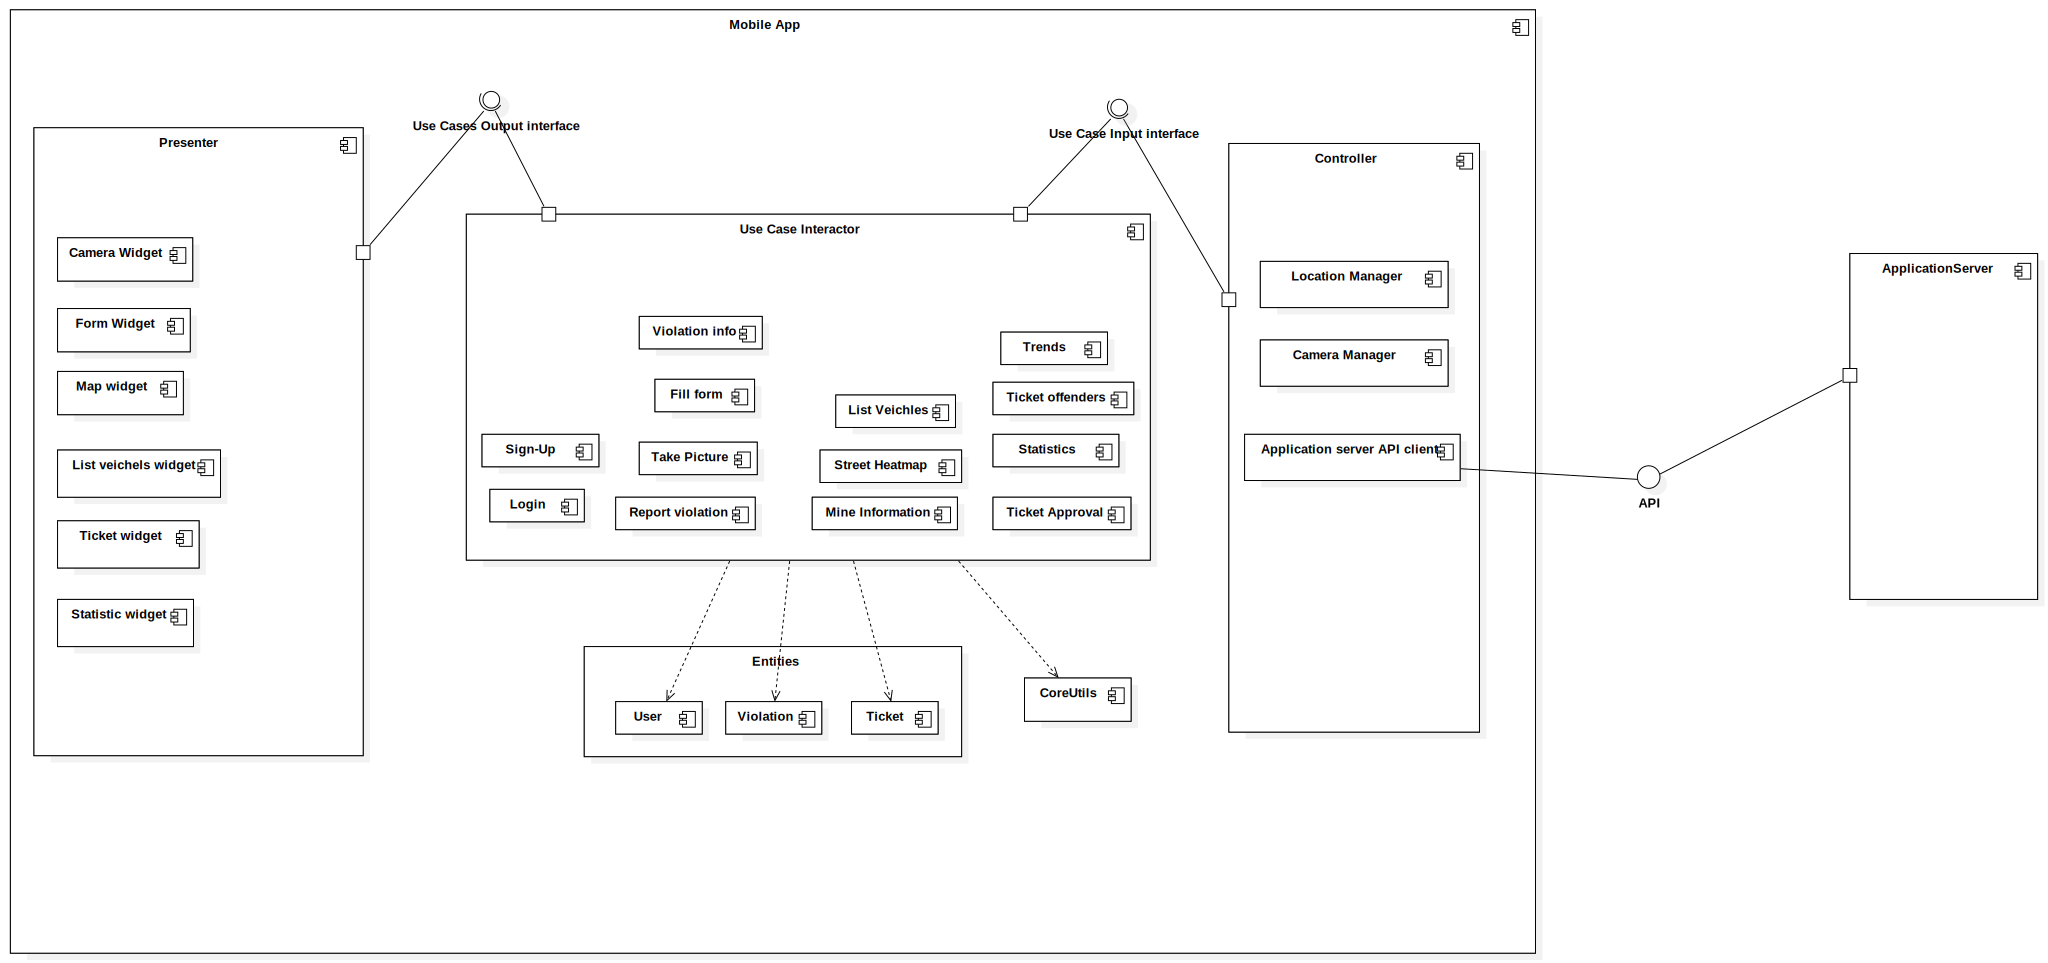
\includegraphics[width=\textwidth]{Images/ComponentDiagram1.png}
\caption{\label{fig:compdiag1} Component diagram for Mobile Application}
\end{sidewaysfigure}

Figure \ref{fig:compdiag1}

\paragraph{Entities}
Entities are the domain of the system, they represent the business objects of the application. In our case entities are plain objects that don't have any dependency on other part of the system (eg. frameworks).
Since the core of our system is based on \textbf{Users}, \textbf{Violations} and \textbf{Tickets} we have included those entities.

\paragraph{Use Cases}
Use cases are components that represent our system actions, they are pure business logic which describe what is possible to do do with the application. We have one component for every possible use case.

We encapsulate all use case in a \textbf{Use Case interactor} which manages all possible use cases, it depends on the entites and has communication ports with the Controller and Presenter.
In fact the use case interactor has two ports: an input, which interfaces with the Controller and an output port connected with the Presenter. As an example: if there is data coming from the camera, this is acquired by an adapter of the controller and is passed to the Use case interactor which coordinates the Use Cases and the data just acquired. After data is processed, it goes to the Presenter and visulalized by the widgets of the UI.

Here follows the list of every Component of the Use case group. We have to add a note here: when it's written for example that a component interacts with the Application server, it doesn't mean that this component interacts directly with the Application API. As we have written before, every use case has to interact firstly direcly with the controller which handles then the connections with the external interfaces. The same goes for communicating with the UI, every data transfer happens via the Use-Case/Presenter interface. In order to keep the following descriptions short, we just say what the component does in a higher level.


\begin{itemize}
  \item \textbf{Sign-Up}: This component allows to add new users to the system. It has to get the input strings (username, password, user data etc. ) from the sign-up widget, validate them before sending the request to the Application Server. After, it has get the answer from the Server and communicate to the user if the sign-up was successful or not.
  \item \textbf{Login}: This component allows the login to the App. It has to get the input from the Login widget, communicate the strings to the Application Server and interpret the response if the user is autorized to login or not.
  \item \textbf{Take Picture}: This component makes possible to take picture of violations. After the picture has been taken, it has to send it to the Application Server and wait for an asnwer. If the answer is that a plate is found, than it calls the next use case "Send form". If no plates are found it asks the user to take a picture again discarding the previous one. If more than one plate is found, it activates a "brush tool mode" (in the Camera Widget) to ask the user to cover the other plates present in the picture. Then it has to manipulate directly the picture changing the color of the pixels selected by the user. Lastly it can send the picture to the Server.
    \item \textbf{Send form}: This component presents the user the form in which he can choose the type of violation. After the form has been submitted bythe user, it is sent to the Application Server in order to be stored.

  \item \textbf{List Vehicles}:
  \item \textbf{Street Heatmap}:
  \item \textbf{Ticket Approval}:
  \item \textbf{Statistics}:
  \item \textbf{Ticket Offenders}:
  \item \textbf{Trends}
\end{itemize}



\paragraph{CoreUtils}
This component encapsulates all the libraries and classes with methods that can be needed by any use case.
Here we list some of these functions:
\begin{itemize}
  \item Input validation
  \item Error handling and reporting
  \item Exceptions
  \item Data conversion
\end{itemize}

\paragraph{Controller}
The controller component  encapsulates all the specific adapters which are devoted to retrieve and store data from different sources such as the local filesystem, the device sensors, the camera and lastly our application service API which is described in section \ref{API}.
Each component of the controller in fact implements the interfaces required by the use cases.
Here is the description of each sub-component:
\begin{itemize}
  \item \textbf{Location Manager}: this component is responsible of getting the location of the user accessing the libraries of the OS of the device
  \item \textbf{Camera Manager}: this component is responsible of getting access to the camera of the device
  \item \textbf{Application server API client}: this component handles all HTTP request to and from our Application server
\end{itemize}

\paragraph{Presenter}
The presenter is a macro components that includes all the components of the UI.
Here follows the list of every component with the description:
\begin{itemize}
  \item \textbf{Sign-Up}: this components coordinates every page shown in the mobile application, and provides the navigation bar
  \item \textbf{Login Widget} : this is the login page and sig-up
  \item \textbf{Camera Widget}: this shows what is recorded by the camera, has a button for taking pictures, activate zoom and other camera functionalities. It also shows the picture once taken and implements the "brush tool mode"
  \item \textbf{Form Widget}: this shows a list of possible description of violations the user can select
  \item \textbf{Map Widget} : this is responsible for showing the street heatmap
  \item \textbf{List Veicles Widget} : this widget shows the list of vehicles that committed the most violations
  \item \textbf{Ticket Widget}: this shows the list of tickets the authority user can approve or not. It also shows information about each one
  \item \textbf{Statistics widget}: this can show some data visualization about the tickets
\end{itemize}


%%%%%%  APPLICATION SERVER %%%%%%%%%%%%%%%%%%%%%%%%%%%%%%%%%%%%%%%%%%%%%%%%%%%%%%%%%%%%%%%%%%%%%%%%%%%%%%%%%%%%%%%%%%%%%%%%%%%%%%%%%%%%

\subsubsection{Application Server} \label{API}
%%fig  application server
\begin{sidewaysfigure}
\centering
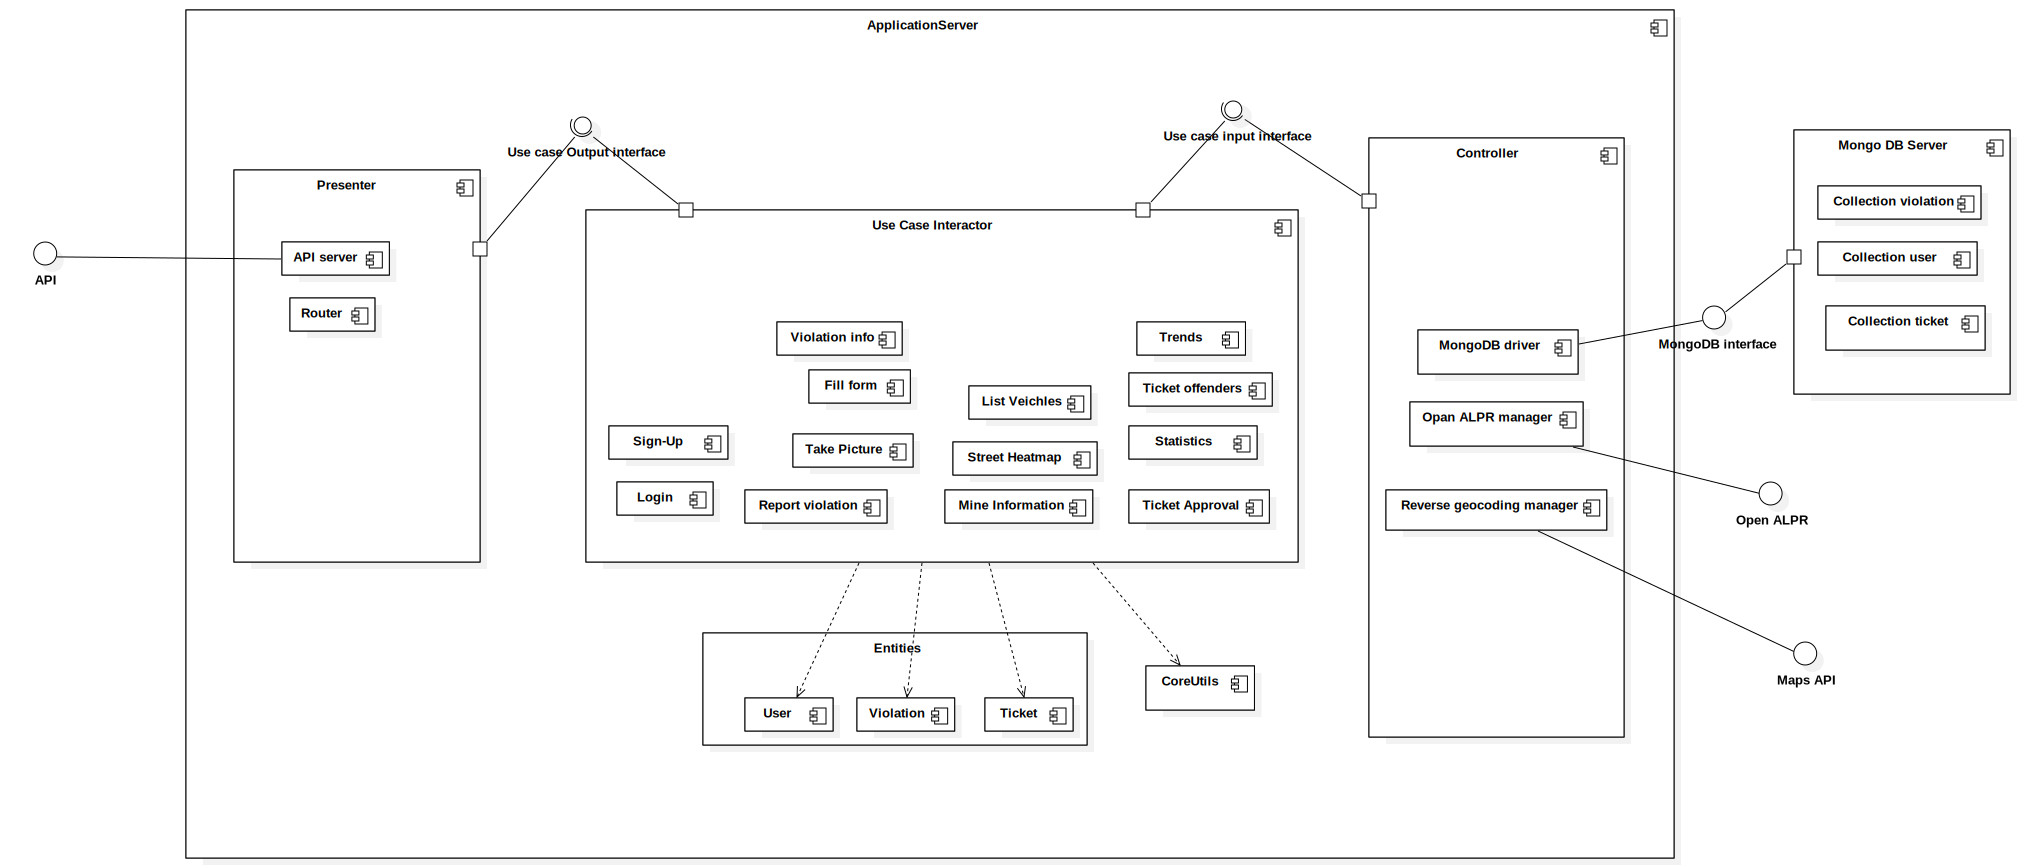
\includegraphics[width=\textwidth]{Images/ComponentDiagram2.png}
\caption{\label{fig:compdiag2} Component diagram for Application Server}
\end{sidewaysfigure}

The architecture of the Application server looks the same as the Mobile Application, but has completly different components in the Presenter and Controller.


\paragraph{Entities}
Entities for the application server are the same as
Since the core of our system is based on \textbf{Users}, \textbf{Violations} and \textbf{Tickets} we have included those entities.


\paragraph{Use Cases}
The use cases components for the server-side have almost the same names as the ones as the application, but they have a completly different logic.
As an example: on the application side we have the use case "Take picture" which has to interact with the device physical camera in order to take the picture and then send it as POST HTTP request to the server, whereas on server side we have the "Get picture" use case, which fetches the HTTP requets, parse the content, send the picture to the OpenALPR service to get the decoded plate and then store the picture.



\paragraph{CoreUtils}
This component encapsulates all the libraries, classes with methods and middleware that can be needed by any use case.
\begin{itemize}
  \item Input validation
  \item Error handling and reporting
  \item Exceptions
  \item Data conversion
  \item Body parser for HTTP requests
\end{itemize}



\paragraph{Controller}


\paragraph{Presenter}
The presenter is the macro components that encapsulates all the frameworks needed to provide an API interface.



\subsection{Deployment view}

In Figure \ref{fig:deploy} is shown the Deployment diagram.

The deployment consist of three main devices. The first tier consist is \textbf{Mobile device} the user will use, which can be a smartphone or a tablet using as operating system either iOS or Android.
The exection environment is the built Flutter app.


The second tier is the \textbf{Application Server}. It is supposed to be a dedicated server running a linux distribution specific for server use. As an example of OS we choose Centos 7. Other distros can be used like Red Hat Enterprise Linux, Debian, OpenSUSE.
As execution enviorment we install Node.js which is an open-source JavaScript runtime environment that executes JavaScript code outside of a browser. Inside Node.js we use the web application framework Express.js which is designed for building web applications and APIs.


The third tier is the \textbf{DB Server}. It consists in another server where we run the DB system MongoDB. We choose to run the database in a separate server and not in the same as the ApplicationServer in order to increase scalability. MongoDB is a cross-platform document-oriented database program. Classified as a NoSQL database program, MongoDB uses JSON-like documents with schema.



\begin{figure}
\centering
\includegraphics[width=\textwidth]{Images/DeploymentDiagram1.png}
\caption{\label{fig:deploy} Deployment diagram}
\end{figure}



\subsection{Runtime view}


A note for the sequence diagrams, we omit that every call to and from a specific use case must pass from the use case interactor to keep it simpler.

\subsubsection{Reporting Violation}

In the following sequence diagram we show the runtime of the function of reporting a violation.
First the user taps to open the page related to violation reporting. The \textbf{page manager} so







\subsection{Selected Architectural styles and patterns}



As already introduced each part of our system will use the Clean Architecture, proposed by Robert C. Martin. We apply this architecture both on the mobile application and in the Application Server.



\begin{figure}
\centering
\includegraphics[width=\textwidth]{Images/cleanArchi.pdf}
\caption{\label{fig:cleanArchi} Clean Architecture \cite{clean} p. 203}
\end{figure}

\subssubection{Dependency Rule}

"The concentric circles in Figure \ref{fig:cleanArchi} represent different areas of software. In general, the further in you go, the higher level the software becomes. The outer circles are mechanisms. The inner circles are policies.
The overriding rule that makes this architecture work is the Dependency Rule:
\textit{Source code dependencies must point only inward, toward higher-level policies.}
Nothing in an inner circle can know anything at all about something in an outer circle. In particular, the name of something declared in an outer circle must not be mentioned by the code in an inner circle. That includes functions, classes, variables, or any other named software entity." \cite{clean}


\subsubsection{Entities}
"Entities encapsulate enterprise-wide Critical Business Rules. An entity can be an object with methods, or it can be a set of data structures and functions. It doesn’t matter so long as the entities are the business objects of the application. They encapsulate the most general and high-level rules. They are the least likely to change when something external changes. For example, you would not expect these objects to be affected by a change to page navigation or security. No operational change to any particular application should affect the entity layer" \cite{clean}


\subsubsection{Use Cases}
"The software in the use cases layer contains application-specific business rules. It encapsulates and implements all of the use cases of the system. These use cases orchestrate the flow of data to and from the entities, and direct those entities to use their Critical Business Rules to achieve the goals of the use case.
We do not expect changes in this layer to affect the entities. We also do not expect this layer to be affected by changes to externalities such as the database, the UI, or any of the common frameworks. The use cases layer is isolated from such concerns.
We do, however, expect that changes to the operation of the application will affect the use cases and, therefore, the software in this layer. If the details of a use case change, then some code in this layer will certainly be affected." \cite{clean}



\subsubsection{Interface Adapters}
"The software in the interface adapters layer is a set of adapters that convert data from the format most convenient for the use cases and entities, to the format most convenient for some external agency such as the database or
the web. The presenters, views, and controllers all belong in the interface adapters layer. The models are likely just data structures that are passed from the controllers to the use cases, and then back from the use cases to the presenters and views." \cite{clean}



\subsubsection{Adantages of Clean architecture}

Following are some reasons which  a good architectural pattern for our app:
\begin{itemize}
  \item All business logic is in a use case, so it’s easy to find and not duplicated anywhere else
  \item Good monolith with clear use cases that you can split in microservices later on

\end{itemize}



\subsubsection{REST}

The communication between the mobile application and the microservice will be done via HTTP requests following REST principles. REST (Representation State Transfer) is an architectural style for communication based on strict use of HTTP request types. One of the most important REST principles is that the interaction between the client and server is stateless between requests. Each request from the client to the server must contain all of the information necessary to understand the request. The client wouldn’t notice if the server were to be restarted at any point between the requests.


\subsection{Other design decisions}
Here we describe the frameworks and languages hat should be used to produca a state-of-art application.

\paragraph{Flutter}


\paragraph{Node.js}
To build a microservice

\subsubsection{MongoDB}
MongoDB is a noSQL database. It stores data as document which can have different shemas.
 \label{cleanArchiref}

This application will be developed with the MVP architectural pattern. In general, the MVP pattern allows separating the presentation layer from the logic, and this feature can be useful when we test the app. MVP is a user interface architectural pattern, which eases automated unit testing and it helps with providing clean code. This pattern consists of three parts which are Model, View and Presenter. In this pattern, model does not communicate with the view directly, it is the Presenter’s responsibility to communicate with the Model and update the View. SafeStreet application will be developed with the MVP architectural pattern in place of the MVC (model, view and controller) because of the test advantage mentioned above and compared to MVVM the architecture does not fit to the project design. MVVM does not give us a relation 1-1 between Presentation and View. For that reason, during this project it is recommended to utilize the MVP architectural pattern. There are more architectural patterns that we considered and discarded, like “Client-server pattern” or “Layered pattern”, but as mentioned above the MVP architecture would be the best fit for the SafeStreet Application.

\begin{figure}
\centering
\includegraphics[width=\textwidth]{Images/MVC.png}
\caption{\label{fig:MVC} MVC Architectural diagram}
\end{figure}

\subsubsection{Model}
The model component stores data and its related logic. It represents data that is being transferred between controller components or any other related business logic. It responds to the request from the views and also responds to instructions from the controller to update itself. It is also the lowest level of the pattern which is responsible for maintaining data. In this project we use MongoDB database to store all the useful data. As well as we will use NODE.JS as the application server to build and run the application.

\subsubsection{View}
A View is that part of the application that represents the presentation of data.
Views are created by the data collected from the model data. A view requests the model to give information so that it resents the output presentation to the user.
In order to implement SafeStreet application we are going to use Flutter framework. Flutter helps app developers build cross-platform apps faster by using a single programming language. Although there are some other frameworks to implement cross-platform apps, according to [https://nevercode.io/blog/flutter-vs-react-native-a-developers-perspective/] Flutter is more efficient than others and has entered the cross-platform mobile development race very strongly.

\subsubsection{Controler}
Controler is the mediator between View and Model which hold responsibilities of everything which has to deal with presentation logic in the application. Presenter does the job of querying the Model, updating the View while responding to the user’s interactions. It monitors Model and talks to View so that they can handle when a particular View needs to be updated and when to not. In this project we will use Representational state transfer (REST) API in order to communicate between View and Model.REST is the software architectural style of the World Wide Web. REST gives a coordinated set of constraints to the design of components in a distributed hypermedia system that can lead to a higher-performing and more maintainable architecture.
To the extent that systems conform to the constraints of REST they can be called RESTful. RESTful systems typically, but not always, communicate over Hypertext Transfer Protocol (HTTP) with the same HTTP verbs (GET, POST, PUT, DELETE, etc.) which web browsers use to retrieve web pages and to send data to remote servers.
We have decided this API because it guarantees to achieve important non-functional requirements such as:
\begin{itemize}
 \item Scalability: every node belonging to our architecture can be multiplied without redesign the whole system.
 \item Portability: Every platform it's able to interact with the server since it's just a matter of HTTP request and JSON response.
 \item Reliability: If suddenly an instance crashes, the load balancer detaches it and will be replaced by a new one automatically.
\end{itemize}

\subsubsection{Why do we use MVP architectural pattern?}

Following are some reasons which makes MVP a good architectural pattern for our app:
\begin{itemize}
\item Makes debugging easier in Applications: MVP enforces three different layers of abstractions which makes it easier to debug your applications. Moreover, since business logic is completely decoupled from View, it is more easier to perform unit testing while developing your application.
\item Enforces better separation of Concerns: MVP does the great job of separating out the business logic and persistence logic out of the Activity and Fragment classes which in turn better enforce good separation of concerns.

\item Code Re-usability: In MVP, the code can be better reused since we can have multiple presenters controlling our Views. This is more important as we definitely don’t want to rely on a single presenter to control our different Views.
\end{itemize}


\subsection{Other design decisions}
